\chapter[Referêncial teórico]{Referêncial teórico}

\section{Agentes}

Existem diferentes definições para agentes. Ainda assim, estas definições possuem conceitos básicos em comum como sugere \cite{mcarthur2007multi}: a noção de agente, seu ambiente e autonomia. Um agente é uma entidade de software ou hardware capaz de reagir de forma autônoma às alterações do ambiente o qual está situado \apud{wooldridge1999intelligent}{mcarthur2007multi}.


Agentes podem ser representadas por seis características ortogonais como sugere a Figura \ref{fig:hexagono}. Trabalhando juntas, tornam o agente mais suceptível a mudanças e robusto. Quanto maior for a área fechada no diagrama, mais "\textit{agent-like}" é aquele componente do sistema \cite{griss2001software}.

\begin{figure}[h!]
    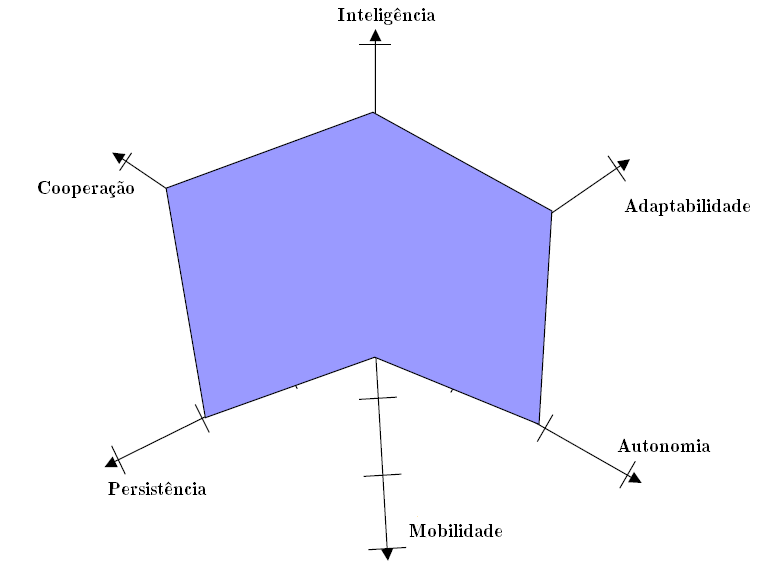
\includegraphics[scale=0.7]{figuras/hexagono_agente}
    \centering
    \caption{Dimensões do agente. Fonte: \cite{griss2001software}. Traduzido.}
    \label{fig:hexagono}
\end{figure}

\section{Sistemas Multiagentes}

Sistemas multiagentes se enquadram no cenário onde coexistem dois ou mais agentes. Seus objetivos individuais  correspondem a subpartes de que do objetivo geral do sistema \cite{mcarthur2007multi}.

Torna-se necessário para um agente representar e raciocinar sobre os outros agentes no ambiente \cite[pág. 887]{van2008handbook}. 


\section{Padrão}

\section{Catálogo de padrões}

Um catálogo de padrões é um conjunto de padrões relacionados; por vezes vagamente ou informalmente relacionados. No catálogo, os padrões são subdividios em categorias abrangentes podendo incluir referências cruzadas entre os padrões \cite{appleton1997}. O catálogo de padrões pode incluir a apresentação da estrutura e organização do padrão, mas normalmente não apresenta algo além da estrutura e das relações mais  facilmente identificáveis \cite{appleton1997}.

A exemplo de \citeauthor{gamma1995} (\citeyear{gamma1995}), foram organizaos 23 padrões de projeto orientado a objetos em um catálogo. Este catálogo descreve boas soluções de software de uso genérico, ou seja, padrões que independem do domínio de aplicação. Os autores utilizaram dois critérios para classificar os padrões de projeto: (i) escopo e (ii) propósito. Assim pôde-se comunicar e exibir as relações entre os padrões.

Portanto, em resumo, para caracterizar um catálogo de padrões deve-se fornecer:

\begin{itemize}
    \item Categorias de padrões;
    \item Critérios de classificação do padrão (em categorias);
    \item Relacionamentos/Referências cruzadas entre padrões.
\end{itemize}

\section{Componente}



De acordo com o SWEBOK (\cite{swebok}) um componente de software é uma unidade independente do software. Esta unidade é compreendida em interfaces e dependências bem definidas. Corroborando com esta ideia, \citeauthor{buschmann2007} define componente como parte independente, destacável e executável de um software. Sua responsabilidade é implementar um serviço específico ou um conjunto de serviços de outros componentes ou clientes. 

Um componente provê uma ou mais interfaces que permitem o acesso aos seus serviços. Podem ser comparados a "blocos de construção" para a estruturação de um sistema. Embora um componente seja independente, componentes podem possuir dependências ou ser compostos de outros componentes. Para \citeauthor{buschmann2007} (\citeyear{buschmann2007}), os componentes podem ser representados como módulos, classes ou um conjunto de funções relacionadas. 

\section{Arquitetura de software}

Arquitetura é a estrutura ou organização de componentes 

\begin{citacao}
"A arquitetura de software é uma descrição dos subsistemas e componentes de um sistema de software e as relações entre eles. Subsistemas e componentes são muitas vezes especificados por meio de diferentes pontos de vista para mostrar as propriedades funcionais e não funcionais relevantes de um sistema de software. A arquitetura de um sistema de software é um artefato que resulta de atividades de projeto de software \cite{buschmann2007}."
\end{citacao}

\section{Arquitetura de Sistemas Multiagentes}



